\section{Aufbau und Generierung der Irradiance Map} % (fold)
\label{sec:aufbau_und_generierung_der_irradiance_map}

	Dieses Kapitel wird die eigentliche Datenstruktur und den Generator der Irradiance Map einführen.
	Durch die bisher genannten Definitonen und Verfahren ist man in der Lage, die Irradianz einer Szene für beliebige Oberflächenpunkte und Wellenlängen bis zu einem gewissen Fehler zu ermitteln.
	Es wird darum gehen, eine endliche Anzahl von Punkten auf der Oberfläche auszuwählen und deren Irradianz zu bestimmen.
	Aus den erhaltenen Werten soll dann eine einfach zu bestimmende approximierte Irradianz erstellt werden.
	Wenn nicht anders behauptet, verwenden wir in diesem Kapitel wieder die bereits eingeführten Variablen des vorigen Kapitels.

	\subsection{Ein Rückblick auf Vertex Lighting} % (fold)
	\label{sub:rückblick_auf_vertex_lighting}

		Im letzten Kapitel wurde die Irradianz $R$ der Szene $\Sigma$ nur an den Eckpunkten der Mesh evaluiert und gespeichert.
		Für Punkte im Inneren von Dreiecken führten wir eine lineare Interpolation durch.
		Die Approximation $\tilde{R}(x,\lambda)$ des Wertes $R(x,\lambda)$ für einen Punkt $x\in\e{T}$, der in einem Dreieck $(A,B,C)$ mit den baryzentrischen Koordinaten $(u,v,w)$ lag, und einer Wellenlänge $\lambda\in (0,\infty)$ beschrieben wir durch die folgende Definition.
		\[
			\tilde{R}(x,\lambda) \define w R(A,\lambda) + u R(B,\lambda) + v R(C,\lambda)
		\]
		Dieses Verfahren wird auch \enquote{Vertex Lighting} genannt und findet häufige Anwendungen in der Computerspieleindustrie \cite{tricks-game}.
		Vor allem bei der \enquote{Dragon}-Szene reichte diese Form der Intepolation aus, weil alle Dreiecke der Mesh klein genug waren, um den Verlauf der Irradianz gut zu beschreiben (siehe Abbildungen \ref{fig:irr-est-ra-dragon} und \ref{fig:irr-est-ra-dragon2}).
		Allerdings kam es bereits in der \enquote{Shaderball}-Szene zu ersten Interpolationsartefakten, wie in Abbildung \ref{fig:irr-est-ra-shaderball2} beim Übergang des Fußes in den Boden zu sehen ist.
		Solche Fehler treten immer dann auf, wenn zwischen zwei Eckpunkten eine unstetige oder extrem schnelle Änderung der Beleuchtung stattfindet.
		Ein typisches Beispiel dafür ist eine als Wand dienende Ebene, die die Szene in zwei Halbräume teilt.
		Abbildung \ref{fig:vertex-lighting-error} beschreibt das Phänomen anhand zweier Skizzen.
		Abbildung \ref{fig:irrmap-cornell} zeigt es zudem in der Praxis für die \enquote{Cornell Box}-Szene.
		\ref{subfig:irrmap-cornell-vmap} weist im Inneren der Box im Gegensatz zu \ref{subfig:irrmap-cornell-ref} fast keinen Schattenverlauf auf.
		\ref{subfig:irrmap-cornell-irrmap} zeigt, dass die später eingeführte Irradiance Map in der Lage ist, diese Fehler zu kompensieren.

		\begin{figure}[h]
			\begin{subfigure}[t]{0.4\textwidth}
				\center
				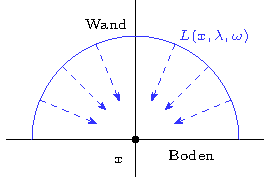
\includegraphics{gg_fig/vertex_lighting-error_1.pdf}
				\caption{Fehlerhafte Messung}
				\label{subfig:vertex-lighting-error-measurement}
			\end{subfigure}
			\begin{subfigure}[t]{0.6\textwidth}
				\center
				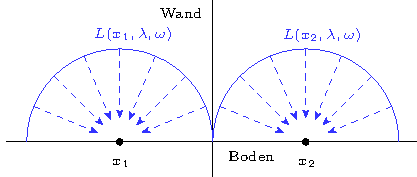
\includegraphics{gg_fig/vertex_lighting-error_2.pdf}
				\caption{Fehlerhafte Intepolation}
				\label{subfig:vertex-lighting-error-interpolation}
			\end{subfigure}
			\caption[Fehlerursachen des Vertex Lighting]{Die Skizzen erklären die Ursachen der beim Vertex Lighting auftretenden Flecken und Artefakte am Beispiel einer Szene, die durch eine Ebene zweigeteilt wird. In \ref{subfig:vertex-lighting-error-measurement} befindet sich der Messpunkt $x$ auf der Ebene. Er kann somit Licht von beiden Seiten der Ebene empfangen und wird in der späteren Interpolation keinen Schattenverlauf aufweisen. In \ref{subfig:vertex-lighting-error-interpolation} befinden sich die Messpunkte $x_1$ und $x_2$ auf jeweils einer Seite der Ebene. Beide empfangen damit das Licht nur von einer Seite. Die Interpolation zwischen den Punkten findet aber über die Wand hinweg statt, was zu sogenannten \enquote{Light Leaks} führt.}
			\label{fig:vertex-lighting-error}
		\end{figure}

		\begin{figure}[h]
			\begin{subfigure}[b]{0.33\textwidth}
				\center
				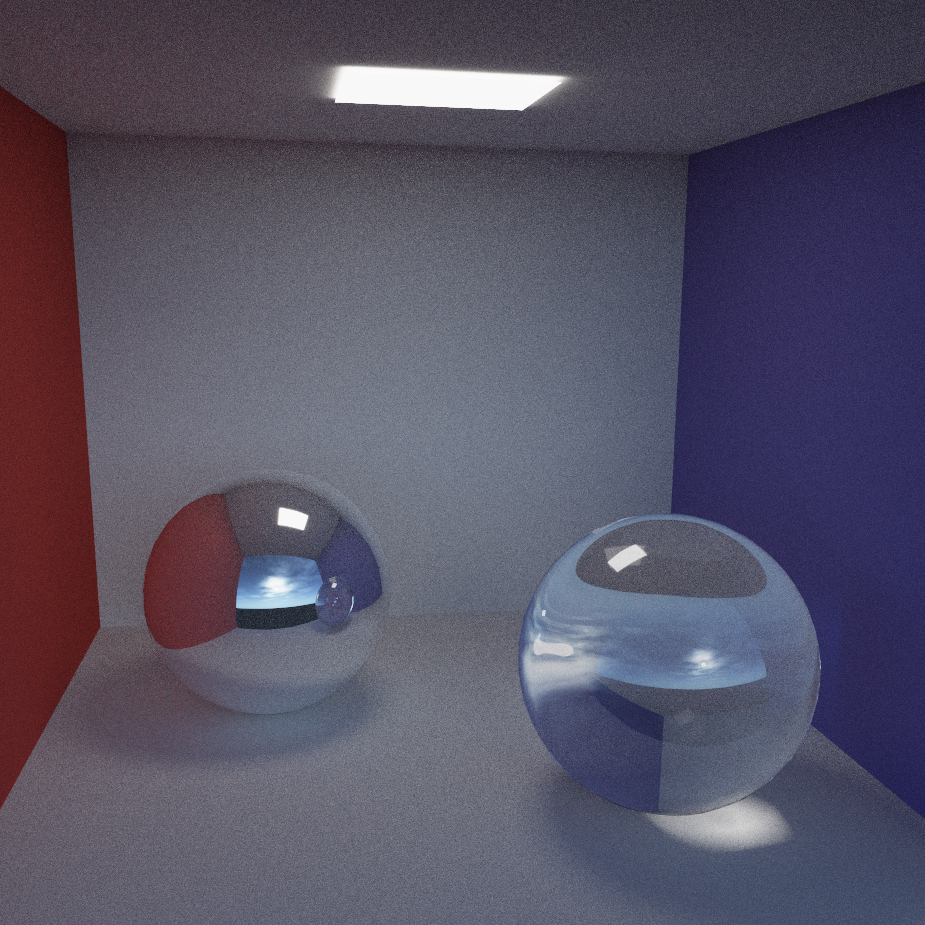
\includegraphics[width=0.95\textwidth]{pic/irrmap-cornell-ref.png}
				\caption{Path Tracing}
				\label{subfig:irrmap-cornell-ref}
			\end{subfigure}
			\begin{subfigure}[b]{0.33\textwidth}
				\center
				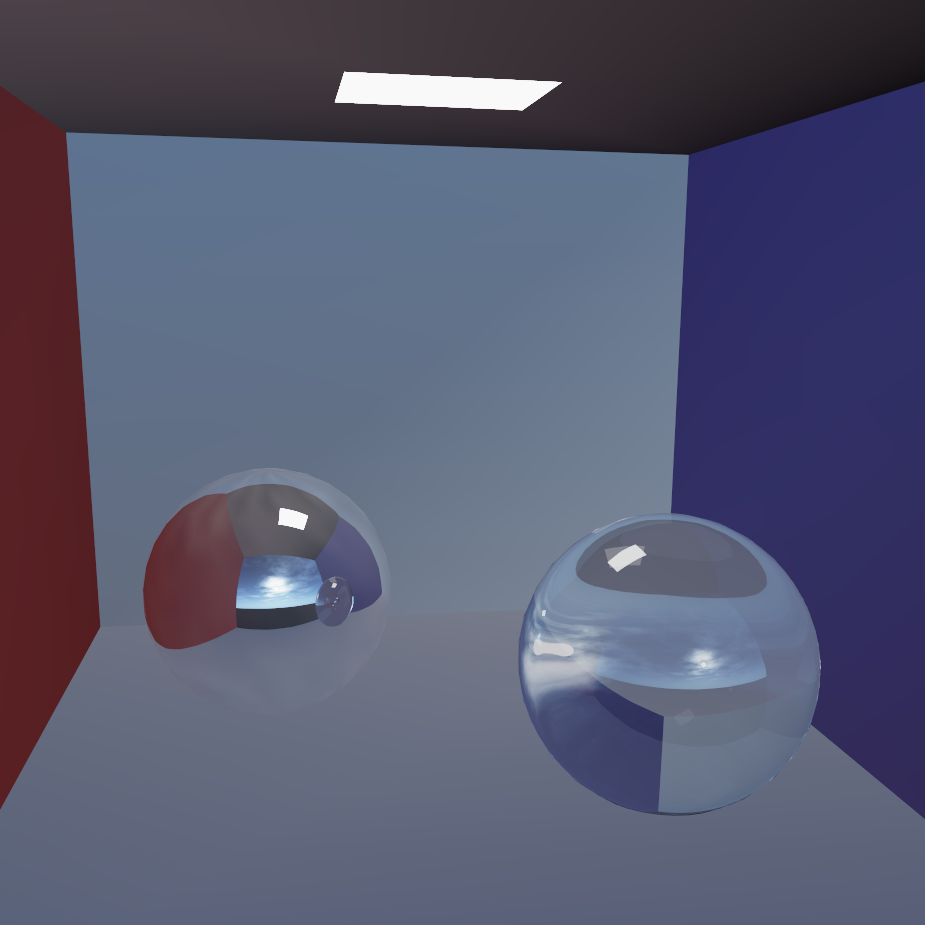
\includegraphics[width=0.95\textwidth]{pic/irrmap-cornell-vmap.png}
				\caption{Vertex Lighting}
				\label{subfig:irrmap-cornell-vmap}
			\end{subfigure}
			\begin{subfigure}[b]{0.33\textwidth}
				\center
				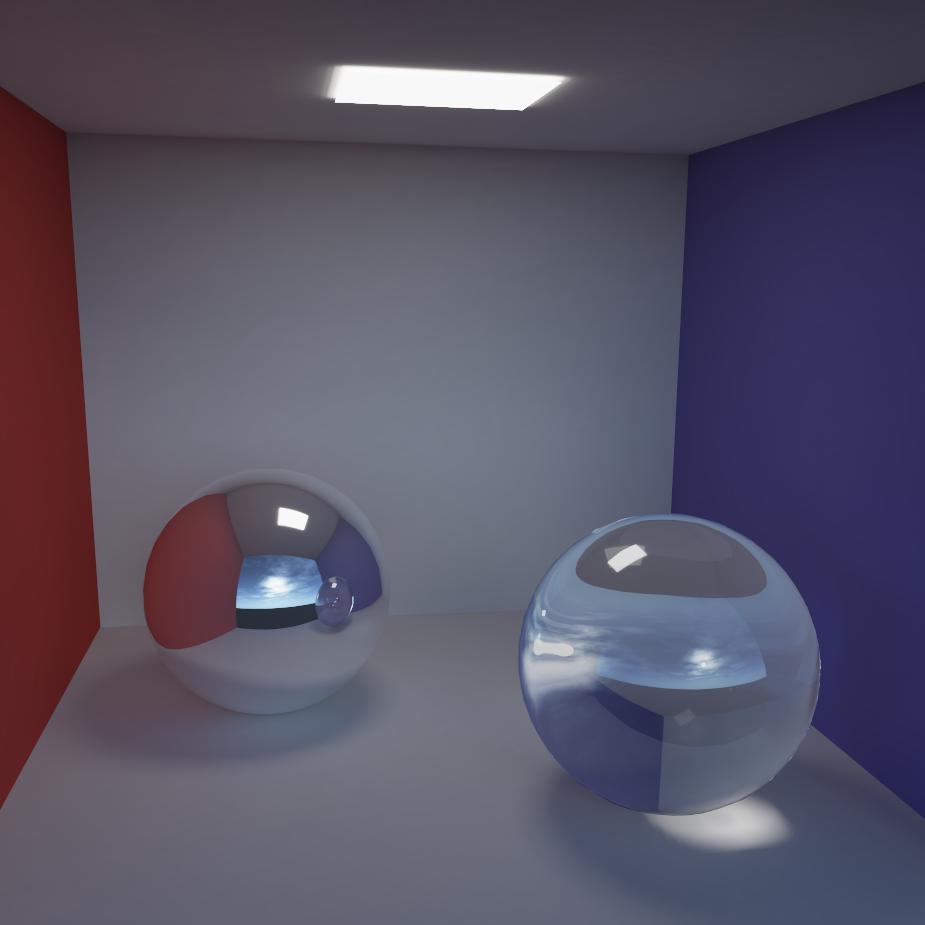
\includegraphics[width=0.95\textwidth]{pic/irrmap-cornell-irrmap.png}
				\caption{Irradiance Map}
				\label{subfig:irrmap-cornell-irrmap}
			\end{subfigure}
			\caption[Irradiance-Map anhand der \enquote{Cornell Box}-Szene]{Die Bilder zeigen die \enquote{Cornell Box}-Szene mit der \enquote{Sky 10}-HDR unter Verwendung von Path Tracing als Referenzbild, von Vertex Lighting und der Irradiance Map. Aufgrund der geringen Auflösung der Mesh ist Vertex Lighting nicht in der Lage die Irradianz der Szene ausreichend zu approximieren. Für die adaptive Irradianzschätzung wurden eine obere Fehlerschranke von $1\unit{\%}$ und maximal $2^{18}$ Samples verwendet. Die Irradiance Map wurde durch circa $278000$ Messpunkte bestimmt, die insgesamt $1.06\unit{MiB}$ einnehmen. Die Berechnungszeit betrug $5120\unit{s}$.}
			\label{fig:irrmap-cornell}
		\end{figure}

		Die genannten Probleme des Vertex Lighting lassen sich nicht komplett durch eine approximierte Irradianz beheben.
		Jede Form der Interpolation benötigt eine endliche Anzahl von aufgenommenen Messpunkten.
		Für jede solcher Mengen von Messpunkten treten aber dieselben beiden Phänomene auf.
		Das Ziel besteht also darin den Fehler durch die Positionierung der Messpunkte sehr klein zu halten, da eine Beseitigung unmöglich ist.
		Im Falle die teilenden Wand aus Abbildung \ref{fig:vertex-lighting-error} würde dies bedeuten, die Punkte $x_1$ und $x_2$ so dicht wie möglich an die Wand, aber nicht auf die Wand zu setzen.

	% subsection rückblick_auf_vertex_lighting (end)

	\subsection{Datenstruktur der Irradiance Map} % (fold)
	\label{sub:datenstruktur_der_irradiance_map}

		Um genauere Approximationen zu ermöglichen, benötigen wir nicht nur Messpunkte an den Eckpunkten der Dreiecke, sondern auch im Inneren dieser.
		Eine Variante die Anforderung zu erfüllen, besteht in der Verwendung von \enquote{Mesh Colors} \cite{mesh-colors}.
		Bei diesem Verfahren speichert man die aufgenommenen Werte an regelmäßigen Punkten des Dreiecks.
		Für jedes Dreieck gibt es dabei eine gewisse Freiheit in der Wahl der Anzahl dieser Punkte, die wir \enquote{Ordnung} nennen.
		Das führt dazu, dass nur dann viele Messpunkte gespeichert werden, wenn in einem Dreieck eine starke Änderung des Irradianzverlaufs auftritt.
		Insbesondere erlaubt die regelmäßige Verteilung der Messpunkte einen schnellen und einfachen Zugriff auf diese durch Verwendung der baryzentrischen Koordinaten eines Punktes.
		Beim Raytracing ist es üblich und meistens auch nötig die baryzentrischen Koordinaten des Schnittpunktes eines Strahls mit einem Dreieck zu berechnen \cite{ray-triangle-intersection}.
		Die Datenstruktur eignet sich damit vor allem für Algorithmen, die, wie Path Tracing in unserem Falle, auf Raytracing basieren.
		In Abbildung \ref{fig:scheme-irr-map} werden die Verteilungen der Messpunkte für verschiedene Ordnungen gezeigt.

		\begin{figure}[h]
			\begin{subfigure}[t]{0.33\textwidth}
				\center
				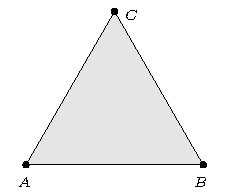
\includegraphics{gg_fig/irr_map_ds-order_1.pdf}
				\caption{\parbox[t]{0.5\textwidth}{Ordnung: $1$ \\ Samples: $3$}}
				\label{subfig:scheme-irr-map-order1}
			\end{subfigure}
			\begin{subfigure}[t]{0.33\textwidth}
				\center
				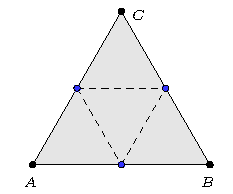
\includegraphics{gg_fig/irr_map_ds-order_2.pdf}
				\caption{\parbox[t]{0.5\textwidth}{Ordnung: $2$ \\ Samples: $6$}}
				\label{subfig:scheme-irr-map-order2}
			\end{subfigure}
			\begin{subfigure}[t]{0.33\textwidth}
				\center
				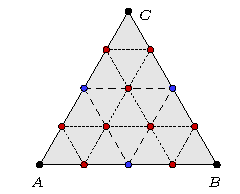
\includegraphics{gg_fig/irr_map_ds-order_4.pdf}
				\caption{\parbox[t]{0.5\textwidth}{Ordnung: $4$ \\ Samples: $15$}}
				\label{subfig:scheme-irr-map-order4}
			\end{subfigure}
			\caption{Die Skizzen zeigen die Datenstruktur der Irradiance Map auf einem Dreieck $(A,B,C)$ für verschiedene Ordnungen. \ref{subfig:scheme-irr-map-order1} speichert Messpunkte nur an den Eckpunkten des Dreiecks. \ref{subfig:scheme-irr-map-order2} speichert zusätzlich noch Messpunkte auf dessen Kante. Erst für Ordnungen größer gleich $3$ werden Messpunkte auch im Inneren des Dreiecks aufgenommen, wie in \ref{subfig:scheme-irr-map-order4} zu sehen ist.}
			\label{fig:scheme-irr-map}
		\end{figure}

		In Abbildung \ref{fig:scheme-irr-map} wird deutlich, dass einige Messpunkte direkt auf den Kanten und Ecken der Dreiecke gespeichert werden.
		Um aber die Fehler des Vertex Lighting aus Abbildung \ref{fig:vertex-lighting-error} zu minimieren, sollte eine Evaluierung der Messwerte nicht an Kanten und Ecken erfolgen.
		Um dies zu gewährleisten, werden wir später die Messwerte im Inneren des Dreiecks schätzen und dann am Rand oder den Ecken speichern.
		Dies wird einen systematischen Fehler der Approximation zur Folge haben.
		Die Verschiebung muss demnach im Vergleich zur Größe des Dreiecks klein sein.
		Die folgende Definition führt das Schema der Abbildung \ref{fig:scheme-irr-map} genauer ein und beschreibt zusätzlich eine Abbildung in den Speicher des Computers.
		\begin{definition}[Irradiance Map auf Dreieck]
			Es seien ein Dreieck $\triangle$ gegeben durch die Sequenz $(A,B,C)$ in $\SR^3$ und $n\in\SN$.
			Dann definiert man die Ordnungsfunktion $s$, die Grundindexmenge $U_n$, die Speicherindexmenge $I_n$, die Speicherindex-Funktion $m_n$ und die Positionsfunktion $p_n$ wie folgt.
			\[
				\func{s}{\SN}{\SN},\qquad s(k)\define \frac{(k+1)(k+2)}{2}
			\]
			\[
				U_n\define \set[u+v\leq n]{(u,v)\in\SN_0^2},\qquad I_n\define \set[i < s(n)]{i\in\SN_0}
			\]
			\[
				\func{m_n}{U_n}{I_n},\qquad m_n(u,v) \define \frac{(u+v)(u+v+1)}{2} + v
			\]
			\[
				\func{p_n}{U_n}{\triangle},\qquad p_n(u,v)\define \triangle\curvb{\frac{u}{n},\frac{v}{n}}
			\]
			Eine Irradiance Map der Ordnung $n$ auf $\triangle$ ist gegeben durch eine Abbildung $\func{f}{\im p_n}{\triangle}$.
			Wir nennen $s(n)$ die Größe von $f$.
		\end{definition}

		Der Definitionsbereich einer Irradiance Map besteht genau aus den markierten Punkten des Dreiecks aus Abbildung \ref{fig:scheme-irr-map}.
		$U_n$,$I_n$ und $m_n$ bieten eine Möglichkeit diese Menge durch Index-$uv$-Koordinaten zu indizieren und in den Speicher abzubilden.
		Um eine explizite Vorstellung dieser drei Konstrukte zu bekommen, zeigt Abbildung \ref{fig:scheme-irr-map-memidx} sie anhand der Ordungen $2$ und $4$.
		$p_n$ transformiert die jeweiligen Index-$uv$-Koordinaten in eine Position auf dem Dreieck.

		\begin{figure}[h]
			\begin{subfigure}[t]{0.5\textwidth}
				\center
				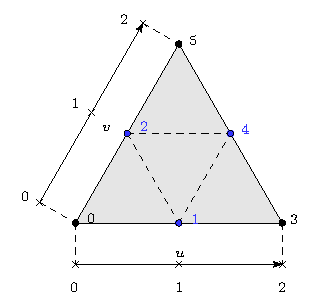
\includegraphics{gg_fig/irr_map_memidx-order_2.pdf}
				\caption{Ordnung: $2$}
			\end{subfigure}
			\begin{subfigure}[t]{0.5\textwidth}
				\center
				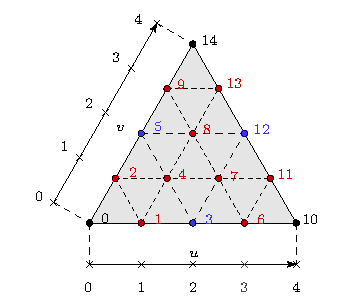
\includegraphics{gg_fig/irr_map_memidx-order_4.pdf}
				\caption{Ordnung: $4$}
			\end{subfigure}
			\caption{Die Skizzen zeigen die Datenstruktur der Irradiance Map auf einem Dreieck für verschiedene Ordnungen $n\in\SN$. Neben jedem Messpunkt $x\in\im p_n$ befindet sich der zugehörige Speicherindex $m_n\curvb{\inv{p}_n(x)}$. Für die Bestimmung der Index-$uv$-Koordinaten wurden deren Koordinatenachsen eingezeichnet.}
			\label{fig:scheme-irr-map-memidx}
		\end{figure}

		Im noch folgenden Irradiance Map Generator wollen wir nach der Bestimmung einer Irradiance Map der Ordnung $n\in\SN$ die Möglichkeit haben, diese durch weitere Messpunkte zu verfeinern, sodass die vorherigen Messpunkte nicht umsonst aufgenommen wurden.
		Solch eine Verfeinerung oder auch Fortsetzung ist nicht für beliebige zwei Ordnungen möglich.
		In Abbildung \ref{fig:scheme-irr-map-memidx} ist jedoch zu sehen, dass die Verdopplung der Ordnung eine derartige Möglichkeit bietet.
		Es ist auch zu sehen, dass zum Beispiel der Messpunkt mit Index $4$ der Ordnung $2$ auf den Index $12$ der Ordnung $4$ abbgebildet werden muss.
		Auch die Verfeinerung und die Verschiebung des Speicherindex wollen wir durch die folgende Definition spezifizieren.
		\begin{definition}[Irradiance Map Verfeinerung]
			Sei $f$ eine Irradiance Map der Ordnung $n\in\SN$ auf einem Dreieck $\triangle$.
			Sei weiterhin $r\in\SN$.
			Dann ist eine Irradiance Map $g$ der Ordnung $n\cdot 2^r$ auf $\triangle$ eine Verfeinerung von $f$, wenn
			\[
				g\vert_{\im p_n} = f
			\]
			Die verfeinerte Speicherindex-Funktion ist durch die folgende Definition gegeben.
			\[
				\func{m_{n,r}}{U_n}{I_{n\cdot 2^r}},\qquad m_{n,r}(u,v)\define m_{n\cdot 2^r}(u\cdot 2^r,v\cdot 2^r)
			\]
		\end{definition}

		Der Verfeinerungsgrad $r\in\SN$ in Abbildung \ref{fig:scheme-irr-map-memidx} beträgt gerade $1$, da $2\cdot 2 = 4$.
		Ab einem bestimmten Verfeinerungsgrad wird man genügend Messpunkte aufgenommen haben, sodass die Fehler der Irradianzapproximation auf dem Dreieck gering sein sollten.
		Die Konstruktion der Approximation kann, wie im letzten Kapitel erwähnt, durch verschiedene Interpolationsmethoden und Filter stattfinden.
		Eine allgemeine Formulierung gibt folgende Definition.
		\begin{definition}[Approximierende Irradiance Map Fortsetzung]
			Sei $f$ eine Irradiance Map der Ordnung $n\in\SN$ auf einem Dreieck $\triangle$.
			Dann nennen wir eine Fortsetzung $\func{g}{\triangle}{[0,\infty)}$ von $f$ auf $\triangle$ eine approximierende Fortsetzung von $f$.
		\end{definition}

		Man stellt die Interpolation als eine Fortsetzung der Irradiance Map dar.
		So ist die Datenstruktur selbst unabhängig von der genauen Interpolationsmethode.
		In unserem Falle wird es sich allerdings nur um eine lineare Interpolation in einer Dreieckszelle handeln.
		Man kann sich diese Form der Approximation als eine Verallgemeinerung des Vertex Lighting vorstellen.
		Die gegebene Definition wird durch Abbildung \ref{fig:scheme-irr-map-interpolation} veranschaulicht.
		\begin{definition}[Lineare approximierende Irradiance Map Fortsetzung]
			Seien $f$ eine Irradiance Map der Ordnung $n\in\SN$ auf einem Dreieck $\triangle$ und $g$ eine approximierende Fortsetzung von $f$, sodass für alle $x\in\triangle$ mit den baryzentrischen Koordinaten $(u,v,w)$ das Folgende gilt.
			\[
				g(x) \define
				\begin{cases}
					(1-u_\m{w})f(x_3) + (1-v_\m{w})f(x_1) + (u_\m{w} + v_\m{w} - 1)f(x_2) &: u_\m{w} + v_\m{w} > 1 \\
					u_\m{w} f(x_1) + v_\m{w}f(x_3) + (1-u_\m{w}-v_\m{w})f(x_0) &: \m{sonst}
				\end{cases}
			\]
			\[
				\bar{u}\define \floorb{nu},\qquad \bar{v}\define \floorb{nv},\qquad u_\m{w}\define nu - \bar{u},\qquad v_\m{w}\define nv - \bar{v}
			\]
			\[
				x_0 \define p_n(\bar{u},\bar{v}),\qquad x_1\define p_n(\bar{u}+1,\bar{v}),\qquad x_2\define p_n(\bar{u}+1,\bar{v}+1),\qquad x_3\define p_n(\bar{u},\bar{v}+1)
			\]
		\end{definition}

		\begin{figure}[h]
			\center
			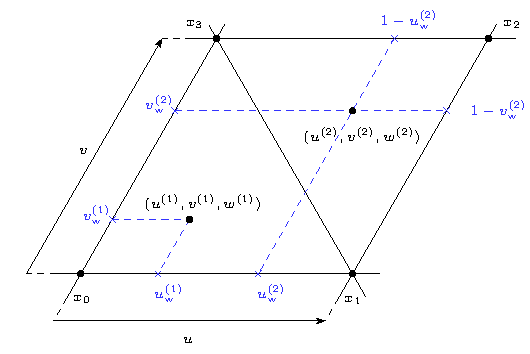
\includegraphics{gg_fig/irr_map_interpolation.pdf}
			\caption{Die Skizze zeigt die in der Definition der Linearen approximierenden Irradiance Map Fortsetzung eingeführten Variablen, um deren Bedeutung zu erläutern. Die Punkte mit den baryzentrischen Koordinaten $(u^{(i)},v^{(i)},w^{(i)}),i\in\set{1,2}$ befinden sich im Inneren eines Dreiecks mit Ordnung $n\in\SN$. Ein Punkt liegt immer in einer Dreieckszelle. Hier sind das entweder $(x_0,x_1,x_3)$ oder $(x_2,x_3,x_1)$. Die Interpolation wird nur durch die Eckpunkte dieser Zelle und den erhaltenen Gewichten $u^{(1)}_\m{w},v^{(1)}_\m{w},u^{(2)}_\m{w},v^{(2)}_\m{w}$ berechnet.}
			\label{fig:scheme-irr-map-interpolation}
		\end{figure}

		Zu beachten ist, dass die Interpolation nur in einem Dreieck stattfindet und nicht auch über mehrere Dreiecke hinweg.
		Für den Fall der linearen Interpolation ist dies auch ausreichend, da wir davon ausgehen, dass Dreiecke, die eine Oberfläche approximieren, an Kanten und Eckpunkten dieselben Messwerte aufweisen oder im sonstigen Fall keine Intepolation stattfinden darf.
		Möchte man aber kompliziertere Interpolationsmethoden verwenden, so ist die Information über Messpunkte in benachbarten Dreiecken unabdingbar.
		Hierfür empfiehlt es sich eine temporäre Datenstruktur zu erzeugen, die die Nachbarschaftsinformationen zwischenspeichert.
		Aus der mit einem anderem Filter erzeugten Irradiance Map lässt sich durch die nochmalige Generierung einer weiteren Irradiance Map mit linearem Filter eine ähnliche Approximation erzielen, die die Nachbarschaftsinformationen nicht mehr benötigt.
		Dieses Verfahren eignet sich vor allem dann, wenn die Generierung von Messpunkten, wie in unserem Falle bei der Irradianzmessung, aufwendig ist und viel Zeit in Anspruch nimmt.
		Der folgende \enquote{C++}-Quelltext implementiert die Irradiance Map Datenstruktur für ein einzelnes Dreieck unter Verwendung aller bisher eingeführten Definitionen.
		\medskip
\begin{tcolorbox}[colframe=black,colbacktitle=white,coltitle=black, attach boxed title to top center={yshift=-2mm},enhanced, titlerule=0.1pt, boxrule=0.5pt, arc=5pt,title=Quelltext:\quad Dreieck Irradiance Map Datenstruktur, breakable]
	\lstinputlisting[style=std,language=c++]{code/irr_map.cpp}
\end{tcolorbox}
\medskip

	% subsection datenstruktur_der_irradiance_map (end)

	\subsection{Irradiance Map Generator} % (fold)
	\label{sub:irradiance_map_generator}

		Die Generierung der Irradiance Map erfolgt durch die Erzeugung der Irradiance Map für jedes Dreieck.
		Da die Szenen im Allgemeinen sehr viele Dreiecke besitzen, ist diese Operation leicht parallelisierbar.

		Die Grundidee bei der Erzeugung besteht in der Verwendung der Verfeinerung einer Irradiance Map.
		Damit man Punkte nicht mehrmals messen muss, behält man die bereits berechneten Messwerte und verdoppelt die Ordnung.
		Für die neu hinzukommenden Messpunkte führt man wieder die Irradianzschätzung durch und wiederholt das Verfahren.
		Auch hier gibt es wieder eine maximale Ordnung, um die Berechnungszeit zu beschränken.
		Um das Verfahren früher abzubrechen, benötigen wir ein Fehlermaß, welches klein bei ausreichenden Approximationen ist.

		Geht man davon aus, dass die Irradianz bezüglich der Wellenlänge $\lambda\in(0,\infty)$ auf dem Dreieck eine gleichmäßig stetige Funktion ist, so konvergiert eine Folge von linear approximierenden Irradiance Map Fortsetzungen $(g_n)_{n\in\SN}$ der Irradiance Maps $f_n,n\in\SN$, sodass $f_{n+1}$ eine Verfeinerung von $f_n$ für alle $n\in\SN$ darstellt, punktweise gegen diese.
		$(g_n(x))_{n\in\SN}$ ist damit für jeden Punkt $x\in\triangle$ auch eine Cauchy-Folge.
		Insbesondere gelten dann die folgenden Aussagen für ein $\varepsilon\in(0,\infty)$.
		\[
			g_n \conv[n\conv\infty] R(\cdot,\lambda)\vert_\triangle,\qquad \abs{g_n(x) - g_m(x)} \conv[n,m\conv\infty] 0
		\]
		\[
			\sup_{x\in\triangle}\abs{g_n(x) - g_m(x)} \conv[n,m\conv\infty] 0,\qquad
			\sup_{x\in\triangle}\frac{\abs{g_n(x) - g_m(x)}}{R(x,\lambda) + \varepsilon} \conv[n,m\conv\infty] 0
		\]
		In der letzten Aussage tritt wieder ein relativer Fehler auf, der in seiner Funktionsweise dem modifizierten Variationskoeffizienten aus Abschnitt \ref{sub:fehler_der_irradianzschaetzung} sehr ähnelt.
		Auch hier wollen wir die Approximation, aufgrund der in diesem Abschnitt genannten Tatsachen, durch einen relativen Fehler bewerten.
		Da man $R(x,\lambda)$ nicht für alle $x\in\triangle$ kennt, betrachten wir den folgenden relativen Fehler $e_{n+1}$ einer Funktion $g_{n+1}$ für $n\in\SN$.
		\[
			e_{n+1} \define \sup_{x\in\im p_{n+1}}\frac{\abs{g_{n+1}(x) - g_{n}(x)}}{R(x,\lambda) + \varepsilon} \conv[n\conv\infty] 0
		\]
		$e_{n+1}$ lässt sich vergleichsweise einfach bestimmen und stellt ein gutes Fehlermaß für die Bewertung der Approximation dar.
		Im Algorithmus werden wir eine Fehlerschranke definieren, die angibt, wann eine berechnete Verfeinerung ausreicht, um so die Rechenzeit weiter zu verkürzen.
		Zu beachten ist, dass mindestens $g_2$ konstruiert werden muss, da $e_1$ nicht definiert ist und keinen Sinn ergeben würde.

		Ein wichtiges Problem besteht allerdings darin, dass sich $R(\cdot,\lambda)$ nur an wenigen Punkten ermitteln lässt, ohne die Berechnungszeit stark zu erhöhen.
		Für hochfrequente Änderungen von $R(\cdot,\lambda)\vert_\triangle$ kann es demnach passieren, dass der relative Fehler eine Approximation gut bewertet, während dies aber nicht der Fall ist.
		Um das Problem zu beheben, ist es entweder notwendig, extrem viele Punkte in $\triangle$ aufzunehmen, um ein besseres Fehlermaß zu erhalten, oder durch weitere einfache Fehlermaße, wie zum Beispiel $d_{n+1}\define \frac{e_{n+1}}{e_n},n\in\SN$, einige solcher auftretenden Fehler zu beseitigen.
		Die Aufnahme einer sehr viel größeren Zahl von Messpunkten, wird zu einem sehr genauen Fehlermaß führen, durch welches eine klare und unverfälschte Bewertung der Approximation möglich ist.
		Auf der anderen Seite ist das Messen der Irradianz ein aufwendiger Prozess, sodass die Berechnung des Fehlers einen immensen Anteil der Rechenzeit einnehmen würde.
		Die Anwendung weiterer Fehlermaße ist meistens einfach zu implementieren und behebt diverse entstehende Fehler.
		Dennoch neigen mehrere Fehlermaße dazu, eine Approximation zu schlecht zu bewerten und resultieren damit auch wieder in einer höheren Berechnungszeit.

		Das beschriebene Verfahren wurde im folgenden \enquote{C++}-Quelltext implementiert.

		\medskip
\begin{tcolorbox}[colframe=black,colbacktitle=white,coltitle=black, attach boxed title to top center={yshift=-2mm},enhanced, titlerule=0.1pt, boxrule=0.5pt, arc=5pt,title=Quelltext:\quad Irradiance Map Generator, breakable]
	\lstinputlisting[style=std,language=c++]{code/gen_irr_map.cpp}
\end{tcolorbox}
\medskip

		Die Abbildungen \ref{fig:irrmap-cornell}, \ref{fig:irrmap-shaderball}, \ref{fig:irrmap-shaderball2}, \ref{fig:irrmap-shaderball-e}, \ref{fig:irrmap-shaderball-e2}, \ref{fig:irrmap-shaderball-e3} und \ref{fig:irrmap-shaderball-e4} zeigen die Ergebnisse des Algorithmus für ausgewählte Szenen.
		In allen Fällen übertrifft die Approximation durch die Irradiance Map das Vertex Lighting Verfahren.
		Deutlich wird dies in Abbildung \ref{fig:irrmap-shaderball}.
		Eine direktionale Lichtquelle lässt sich aufgrund der Unstetigkeit der entstehenden Irradianz im Allgemeinen nur schlecht durch Messpunkte interpolieren.
		Bild \ref{subfig:irrmap-shaderball-vmap} ist durch eine zu geringe Auflösung der Mesh nicht in der Lage, den Kernschatten des Objektes akzeptabel zu approximieren.
		Die Irradiance Map in Bild \ref{subfig:irrmap-shaderball-irrmap} entspricht aber dem Anschein nach dem Referenzbild \ref{subfig:irrmap-shaderball-ref}.
		Erst durch Heranzoomen in Abbildung \ref{fig:irrmap-shaderball2} erkennt man kleine Aliasing-Artefakte am Rand des harten Schattens.
		Die Darstellung der Ordungen der einzelnen Dreieck Irradiance Maps zeigt zudem, dass der Algorithmus nur dann eine höhere Ordung verwendet, wenn eine Änderung der Irradianz, die größer als die gegebene Fehlerschranke ist, gemessen wird.
		Auch für einen vergleichsweise glatten Schattenverlauf in den Abbildungen \ref{fig:irrmap-shaderball-e}, \ref{fig:irrmap-shaderball-e2}, \ref{fig:irrmap-shaderball-e3} und \ref{fig:irrmap-shaderball-e4} erzielt die Irradiance Map bessere Ergebnisse, ohne für jedes Dreieck extrem viele Samples zu verwenden.
		Die durch Vertex Lighting entstehenden Artefakte sind zwar schwach ausgeprägt, können aber dennoch im Vergleich mit den Referenzbildern beobachtet werden.
		In allen Ergebnissen besaß das Vertex Lighting Verfahren jedoch einen großen Vorteil gegenüber der Irradiance Map.
		Die Berechnungszeit von Vertex Lighting betrug immer weniger als $5\unit{\%}$ der Irradiance Map Generierungszeit.

		\begin{figure}[h]
			\begin{subfigure}[t]{0.245\textwidth}
				\center
				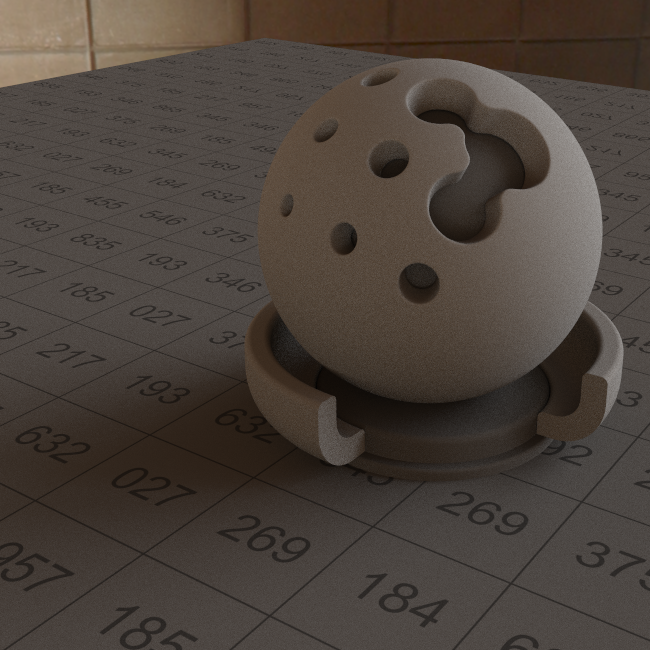
\includegraphics[width=0.95\textwidth]{pic/irrmap-shaderball_e-ref.png}
				\caption{Path Tracing}
			\end{subfigure}
			\begin{subfigure}[t]{0.245\textwidth}
				\center
				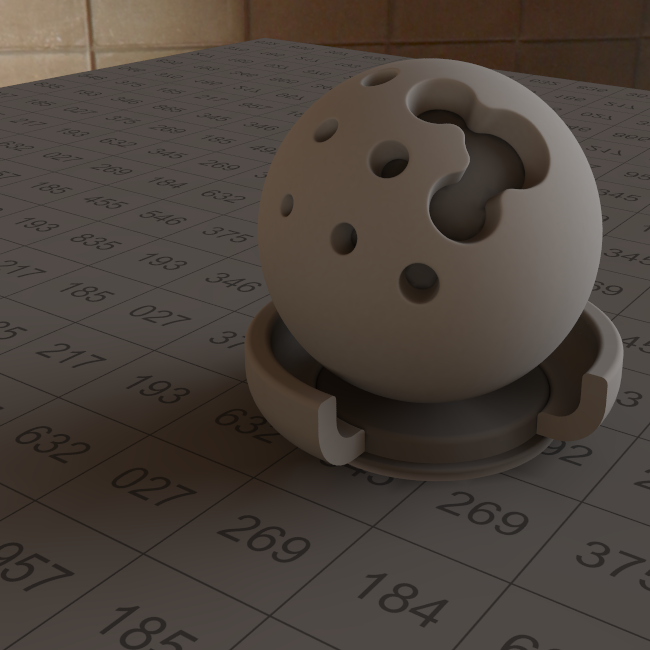
\includegraphics[width=0.95\textwidth]{pic/irrmap-shaderball_e-vmap.png}
				\caption{Vertex Lighting}
			\end{subfigure}
			\begin{subfigure}[t]{0.245\textwidth}
				\center
				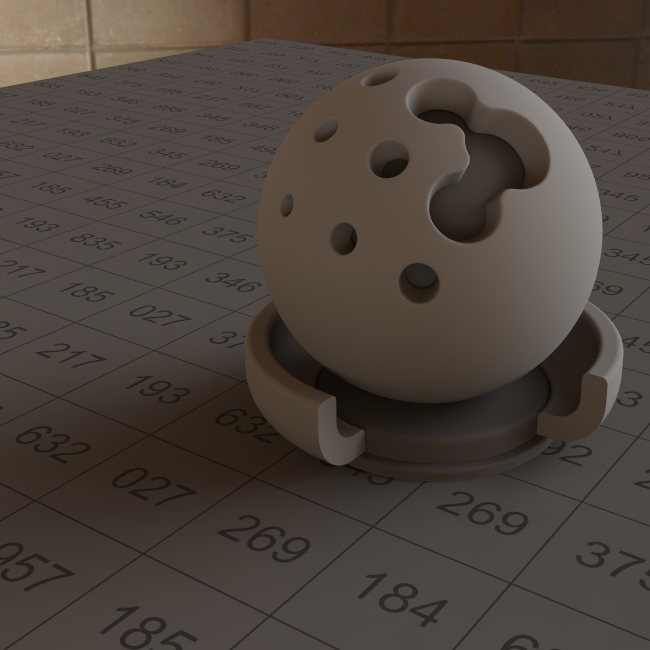
\includegraphics[width=0.95\textwidth]{pic/irrmap-shaderball_e-irrmap.png}
				\caption{Irradiance Map}
			\end{subfigure}
			\begin{subfigure}[t]{0.245\textwidth}
				\center
				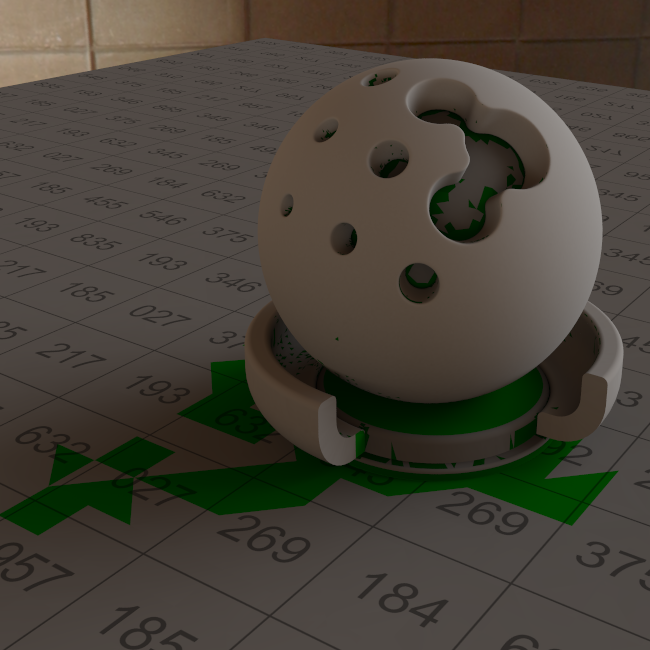
\includegraphics[width=0.95\textwidth]{pic/irrmap-shaderball_e-irrmap-order.png}
				\caption{Irradiance Map Ordnung}
				\label{subfig:irrmap-shaderball-e-irrmap-order}
			\end{subfigure}
			\caption[Irradiance-Map der \enquote{Shaderball}-Szene mit der \enquote{Ennis-Brown House}-HDR]{Die Bilder zeigen die \enquote{Shaderball}-Szene mit der \enquote{Ennis-Brown House}-HDR unter Verwendung von Path Tracing als Referenzbild, von Vertex Lighting und der Irradiance Map. Für die adaptive Irradianzschätzung wurden eine obere Fehlerschranke von $1\unit{\%}$ und maximal $2^{16}$ Samples verwendet. Die Irradiance Map wurde durch circa $9.27\cdot10^6$ Messpunkte bestimmt, die insgesamt $35.4\unit{MiB}$ einnehmen. Die obere Fehlerschranke betrug $10\unit{\%}$ und die maximale Ordnung $2^7$. Die Generierung benötigte $3430\unit{s}$. Die grün markierten Bereich in \ref{subfig:irrmap-shaderball-e-irrmap-order} stellen Dreiecke mit einer Ordnung größer $2$ dar.}
			\label{fig:irrmap-shaderball-e}
		\end{figure}

		\begin{figure}[h]
			\begin{subfigure}[t]{0.33\textwidth}
				\center
				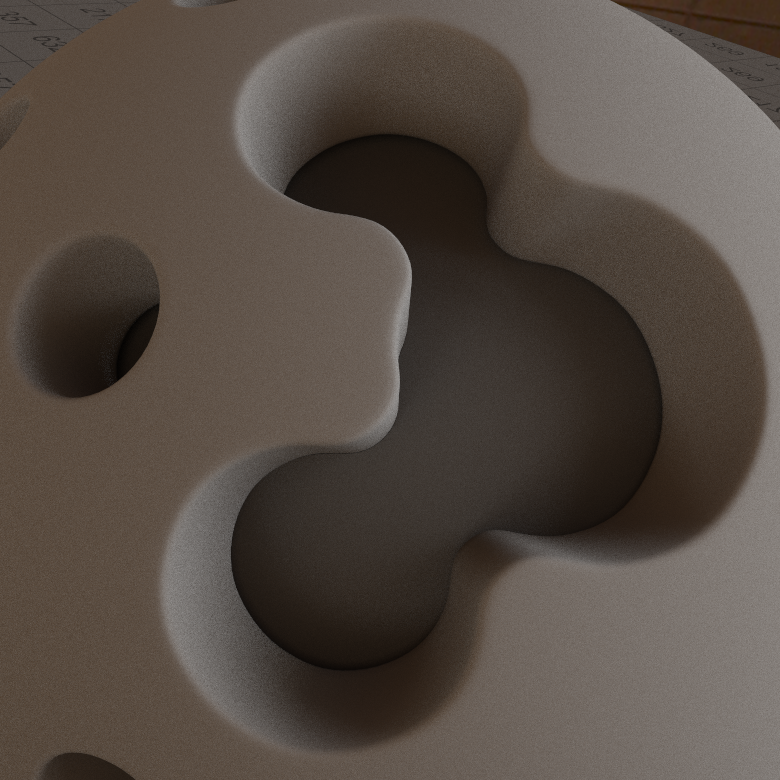
\includegraphics[width=0.95\textwidth]{pic/irrmap-shaderball_e3-ref.png}
				\caption{Path Tracing}
				\label{subfig:irrmap-shaderball-e3-ref}
			\end{subfigure}
			\begin{subfigure}[t]{0.33\textwidth}
				\center
				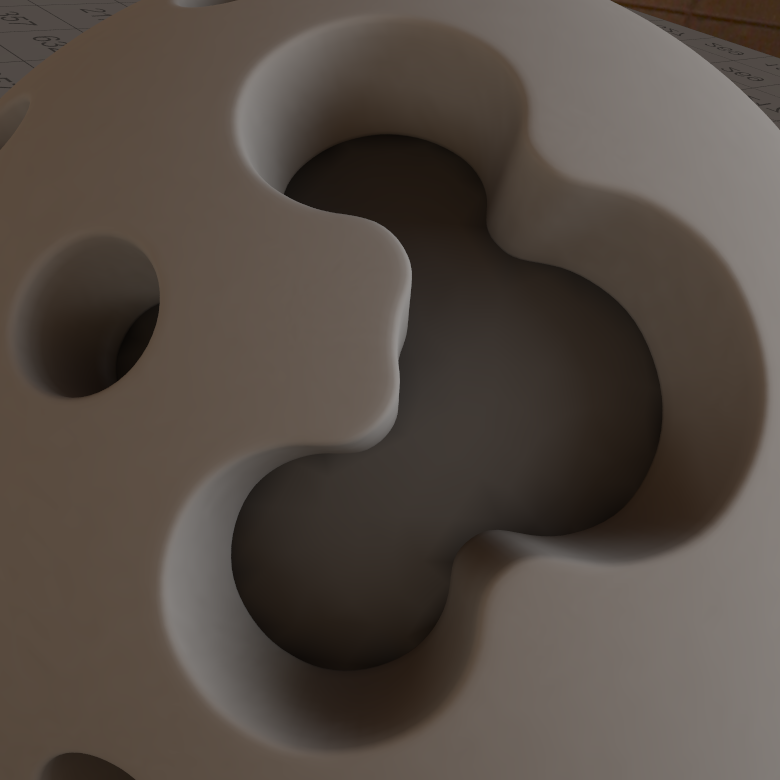
\includegraphics[width=0.95\textwidth]{pic/irrmap-shaderball_e3-vmap.png}
				\caption{Vertex Lighting}
				\label{subfig:irrmap-shaderball-e3-vmap}
			\end{subfigure}
			\begin{subfigure}[t]{0.33\textwidth}
				\center
				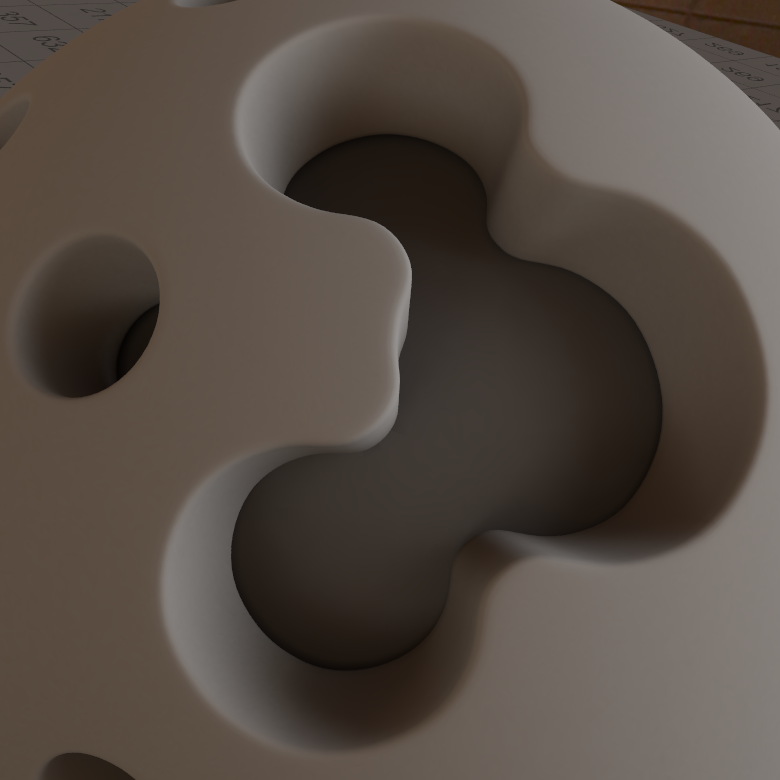
\includegraphics[width=0.95\textwidth]{pic/irrmap-shaderball_e3-irrmap.png}
				\caption{Irradiance Map}
				\label{subfig:irrmap-shaderball-e3-irrmap}
			\end{subfigure}
			\caption[Irradiance-Map der \enquote{Shaderball}-Szene mit der \enquote{Ennis-Brown House}-HDR in den Löchern]{Die Bilder zeigen die oberen Löcher der \enquote{Shaderball}-Szene aus Abbildung \ref{fig:irrmap-shaderball-e}. Die Schattenverläufe in \ref{subfig:irrmap-shaderball-e3-ref} und \ref{subfig:irrmap-shaderball-e3-irrmap} können nicht unterschieden werden. Für Vertex Lighting in \ref{subfig:irrmap-shaderball-e3-vmap} sind am Rand der Löcher Fehler in den Schatten zu sehen.}
			\label{fig:irrmap-shaderball-e3}
		\end{figure}

		\begin{figure}[h]
			\begin{subfigure}[t]{0.33\textwidth}
				\center
				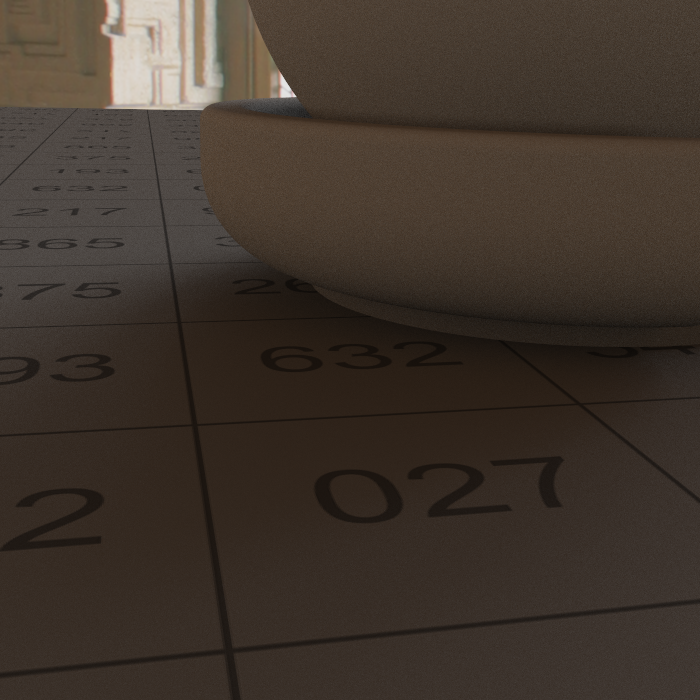
\includegraphics[width=0.95\textwidth]{pic/irrmap-shaderball_e4-ref.png}
				\caption{Path Tracing}
				\label{subfig:irrmap-shaderball-e4-ref}
			\end{subfigure}
			\begin{subfigure}[t]{0.33\textwidth}
				\center
				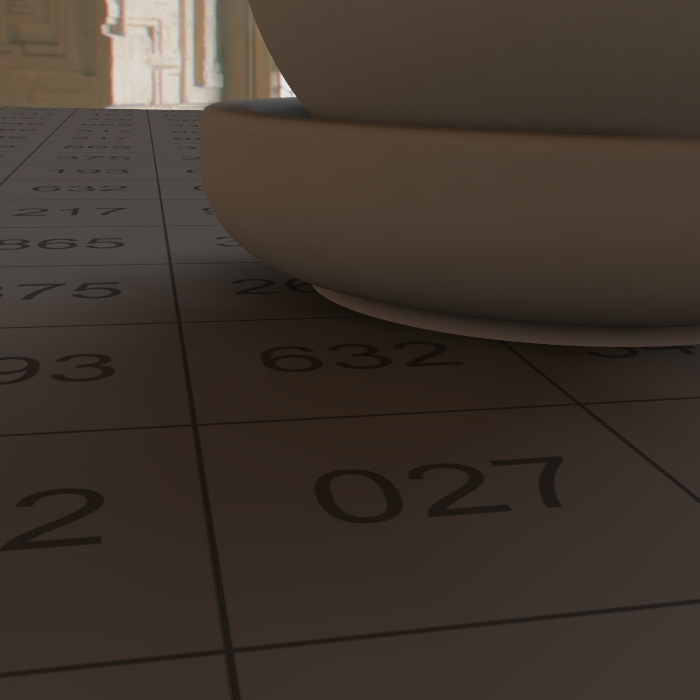
\includegraphics[width=0.95\textwidth]{pic/irrmap-shaderball_e4-vmap.png}
				\caption{Vertex Lighting}
				\label{subfig:irrmap-shaderball-e4-vmap}
			\end{subfigure}
			\begin{subfigure}[t]{0.33\textwidth}
				\center
				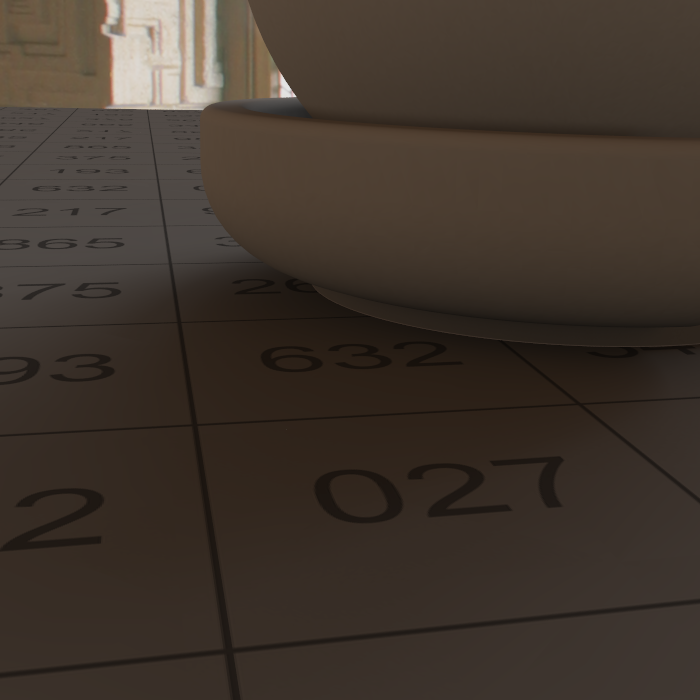
\includegraphics[width=0.95\textwidth]{pic/irrmap-shaderball_e4-irrmap.png}
				\caption{Irradiance Map}
				\label{subfig:irrmap-shaderball-e4-irrmap}
			\end{subfigure}
			\caption[Irradiance-Map der \enquote{Shaderball}-Szene mit der \enquote{Ennis-Brown House}-HDR in den Löchern]{Die Bilder zeigen den Kernschatten der \enquote{Shaderball}-Szene aus Abbildung \ref{fig:irrmap-shaderball-e}. Die Schattenverläufe in \ref{subfig:irrmap-shaderball-e4-ref} und \ref{subfig:irrmap-shaderball-e4-irrmap} können nicht unterschieden werden. Für Vertex Lighting in \ref{subfig:irrmap-shaderball-e4-vmap} sind vor allem am Rand des Schattens kleine Artefakte zu entdecken.}
			\label{fig:irrmap-shaderball-e4}
		\end{figure}

		\begin{figure}[h]
			\begin{subfigure}[t]{\textwidth}
				\center
				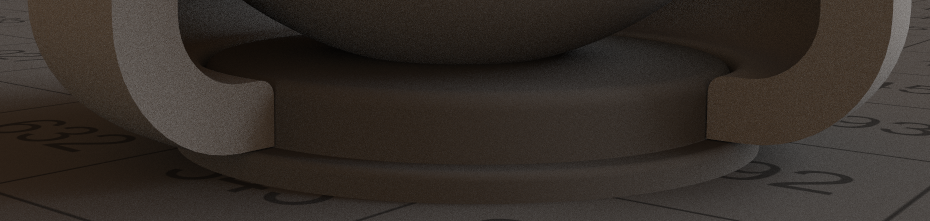
\includegraphics[width=0.95\textwidth]{pic/irrmap-shaderball_e2-ref.png}
				\caption{Path Tracing}
				\label{subfig:irrmap-shaderball-e2-ref}
			\end{subfigure}
			\medskip \\
			\begin{subfigure}[t]{\textwidth}
				\center
				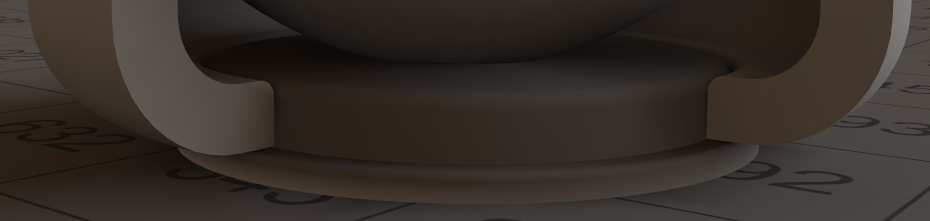
\includegraphics[width=0.95\textwidth]{pic/irrmap-shaderball_e2-vmap.png}
				\caption{Vertex Lighting}
				\label{subfig:irrmap-shaderball-e2-vmap}
			\end{subfigure}
			\medskip \\
			\begin{subfigure}[t]{\textwidth}
				\center
				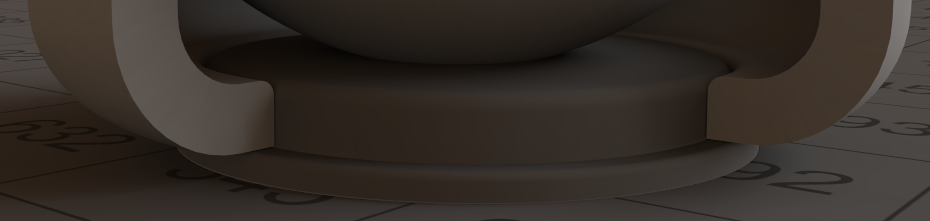
\includegraphics[width=0.95\textwidth]{pic/irrmap-shaderball_e2-irrmap.png}
				\caption{Irradiance Map}
				\label{subfig:irrmap-shaderball-e2-irrmap}
			\end{subfigure}
			\medskip \\
			\begin{subfigure}[t]{\textwidth}
				\center
				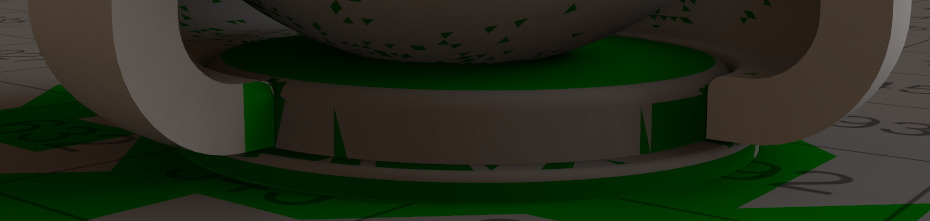
\includegraphics[width=0.95\textwidth]{pic/irrmap-shaderball_e2-irrmap-order.png}
				\caption{Irradiance Map Ordnung}
				\label{subfig:irrmap-shaderball-e2-irrmap-order}
			\end{subfigure}
			\caption[Irradiance-Map der \enquote{Shaderball}-Szene mit der \enquote{Ennis-Brown House}-HDR im unteren Stand]{Die Bilder zeigen den unteren Stand der \enquote{Shaderball}-Szene aus Abbildung \ref{fig:irrmap-shaderball-e}. Die grün markierten Bereiche in \ref{subfig:irrmap-shaderball-e2-irrmap-order} stellen Dreiecke mit einer Ordnung größer $2$ dar. Die Schattenverläufe in \ref{subfig:irrmap-shaderball-e2-ref} und \ref{subfig:irrmap-shaderball-e2-irrmap} können nicht unterschieden werden. Für Vertex Lighting in \ref{subfig:irrmap-shaderball-e2-vmap} ist dies nicht der Fall.}
			\label{fig:irrmap-shaderball-e2}
		\end{figure}

		Die Probleme des verwendeten Fehlermaßes wurden bereits beschrieben.
		Abbildung \ref{fig:irrmap-shaderball2} zeigt das Resultat einer Fehlbewertung.
		Eine der Dreieck Irradiance Maps auf der unteren Platte approximiert den harten Schattenverlauf auf eine extrem schlechte Weise.
		Höchstwahrscheinlich konnten in diesem Dreieck aufgrund der schnellen Änderung der Irradianz nur Messpunkte im Kernschatten aufgenommen werden.
		Die Bewertung durch das Fehlermaß musste demnach positiv ausfallen und die Berechnung beenden.
		In der Praxis ist es allerdings vergleichsweise einfach, die Beleuchtung direktionaler oder anderer singulärer Lichtquellen durch Raytracing und Path Tracing zu simulieren.
		Die Verwendung einer Irradiance Map für singuläre Lichtquellen wie in den Abbildungen \ref{fig:irrmap-shaderball} und \ref{fig:irrmap-shaderball2} ist damit ein unwahrscheinlicher Fall.
		Dennoch zeigt die Szene, das es auch in schwierigeren Situationen möglich ist eine Irradiance Map einzusetzen.


		Im derzeitigen Algorithmus wird für jedes Dreieck die Irradianz an Ecken und Kanten mit einer kleinen Verschiebung in das Innere  geschätzt.
		So werden Fehler der Art aus Abbildung \ref{fig:vertex-lighting-error} verhindert, wie man in Abbildung \ref{fig:irrmap-cornell} anhand der \enquote{Cornell Box}-Szene sehen konnte.
		Die Ergebnisse des Vertex Lighting aus Abschnitt \ref{sub:adaptive_schaetzung_der_irradianz} und Anhang \ref{sec:ergebnisse_adaptive_irradianzschaetzung} zeigen aber, dass diese Fehler nicht bei allen Eckpunkten und Kanten auftreten.
		Ein Großteil der Generierungszeit der Irradiance Map besteht also darin, bereits evaluierte Werte noch einmal zu schätzen.
		Durch eine Analyse der Mesh ist es aber möglich, jedem Eckpunkt und jeder Kante eine Markierung zu geben, die eine Aussage darüber trifft, ob die Irradianz auf dem Eckpunkt beziehungsweise der Kante geschätzte werden darf oder ob sie im Inneren der Dreieck bestimmt werden muss.
		Die Berechnungszeit könnte somit um ein Vielfaches beschleunigt werden.

	% subsection irradiance_map_generator (end)

% section aufbau_und_generierung_der_irradiance_map (end)